\chapter{Results} 

The aim of this project is to create a boundary representation of an indoor environment from laser scan data. This section builds on the literature review and Method and describes the process undertaken to get a B-rep model.\\
\\
The point clouds are processes through an command line program that takes in the point cloud name as a parameter, then saves the B-rep model as an obj file with the same name and same file location as the point cloud.

	\section{Segmentation}
		The segmentation of the point cloud is done with a built in region growing function from Point Cloud Library. A detailed description of the region growing and normal calculation process is given in Section \ref{segmentation-method}.
		
		\subsection{Normal Calculation}
		
		Before segmentation can take place normals need to be calculated for each point in the cloud. Normals are calculated using a Principal components analysis, with the neighbourhood around the point, $k$, set to the nearest 40 points. 
		
		40 was chosen because it gives the best results, higher and the gaps at the corners of the room start to become very big making segments smaller, as well as no co-planar features are detected for example a door will become part of the wall. Any smaller and there is too much variation in the normals making the region growing segmentation leave holes in the planar segments such as in Figure \ref{fig:k=5}:
		
		
		\begin{figure}[H]
			\centering
			\includegraphics[width=1\linewidth]{"Includes/images/Normal Comp/k = 5 ver 2"}
			\caption{$k$ = 5}
			\label{fig:k=5}
		\end{figure}
		
		\begin{figure}[H]
			\centering
			\includegraphics[width=1\linewidth]{"Includes/images/Normal Comp/k = 200 ver 2"}
			\caption{$k$ = 200}
			\label{fig:k=200}
		\end{figure}
		
		Both images are done with the region growing parameters chosen in section \ref{RegionGrowParams}

		
		There is also a speed aspect to the neighbourhood size, smaller results in a much faster computation, and larger much slower. This is not a huge issue as the normal estimation function has multi-threading making it only take up to 10s at most. This is only about 5\% of the total run-time.
		
		
		\subsection{Region Growing}
		\label{RegionGrowParams}
			
		Once the normals have been calculated the point cloud is segmented using region growing. Region growing takes in 5 parameters; Minimum cluster size, Maximum cluster size,Search Method, Number of neighbours, Smoothness threshold and Curvature threshold.
		
		In the case of this project bigger segments are good, so the Maximum cluster size value was never set allowing clusters be as large as the need to be.
		
		The minimum cluster size was set to 5000 points because the chances of a significant wall section being less than 5000 points is very low, having this large number also removes a lot of the clutter in a room. Removing clutter is an important part of this project as any small segment thats not a part of the extent of the room (i.e. walls, roof or floor) will create problems with the rest of the program.
		
		
		\begin{figure}[H]
			\centering
			\includegraphics[width=1\linewidth]{"Includes/images/RegionGrowing/min-size = 100"}
			\caption{Minimum Cluster Size = 100}
			\label{fig:min-size=100}
		\end{figure}
		
		\begin{figure}[H]
			\centering
			\includegraphics[width=1\linewidth]{"Includes/images/RegionGrowing/min-size = 5000"}
			\caption{Minimum Cluster Size = 5000}
			\label{fig:min-size=5000}
		\end{figure}
		
		The Smoothness and Curvature thresholds are very important in this project as the outcome relies on planar segments so strict thresholds on curvature and smoothness are important to make sure that any segment is a planar segment and does not cover two sides of a room. You can see in Figure \ref{fig:NoSmoothCurv} that the roof and right hand wall are one segment, resulting in a fitted plane that goes at a 45\textdegree\: angle through the room. As well as the person in the figure who is large enough to pass all the tests but is most defiantly not a feature that needs to be kept. So because this project relies heavily on planes the Smoothness and Curvature thresholds are strictly set so that only planar segments are kept.
		
		
		\begin{figure}[H]
			\centering
			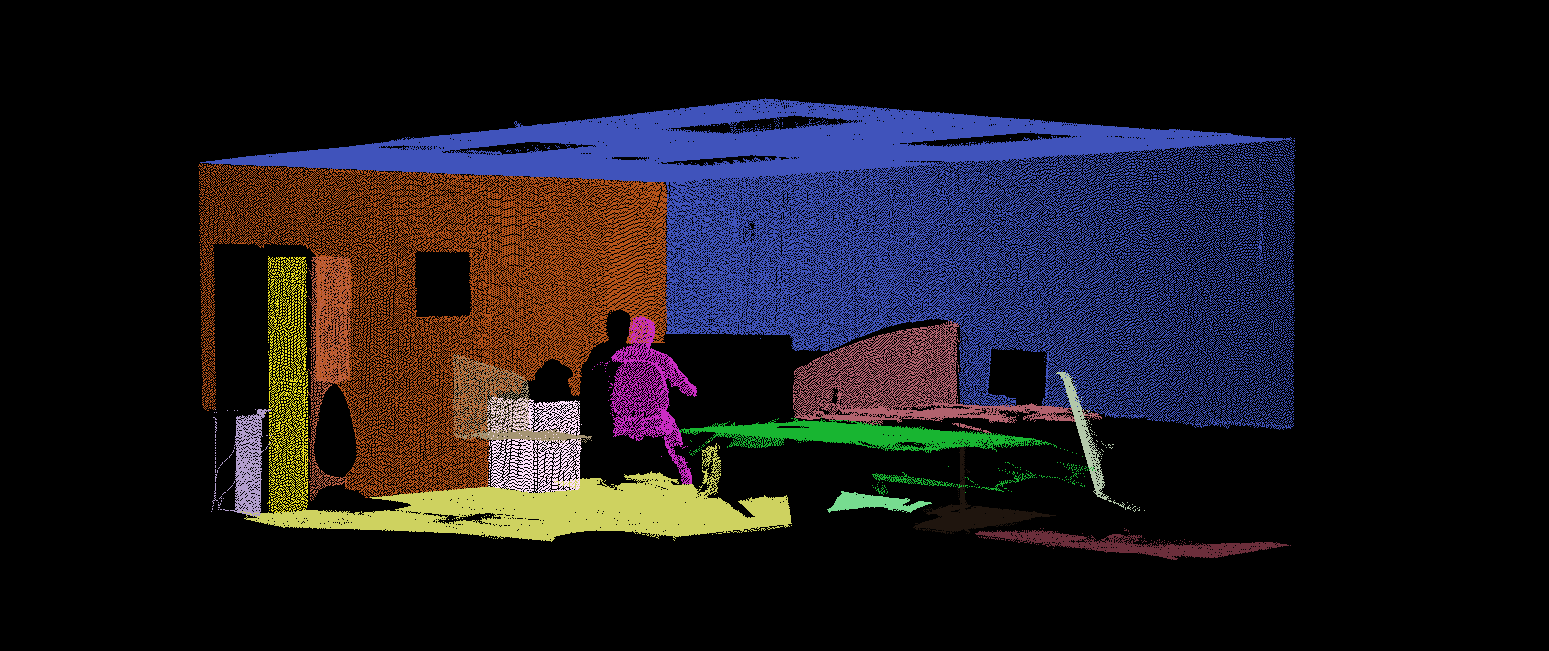
\includegraphics[width=1\linewidth]{Includes/images/RegionGrowing/NoSmoothCurv}
			\caption{Region Growing Run with no Smoothness or Curvature Thresholds set}
			\label{fig:NoSmoothCurv}
		\end{figure}
	
		Number of neighbours and search method in region growing is the same as in the normal computation. The number of neighbours is set to the same value as the normal calculation. the main difference in varying values for number of neighbours is that with a very low value, shown in fig. \ref{fig:neighbours-5}, the door can be seen as a separate segment to the wall and with a large value the door becomes part of the wall. This becomes important later 
		
		
		\begin{figure}[H]
			\centering
			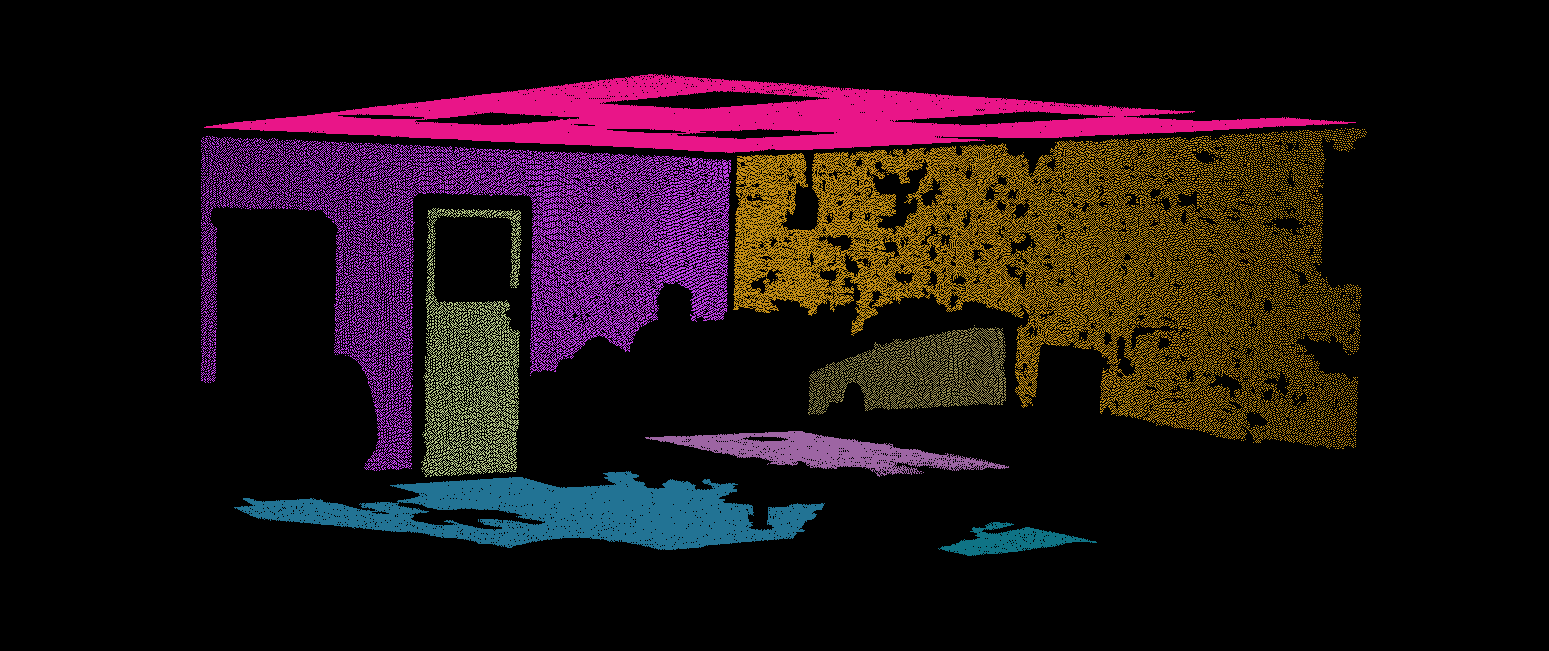
\includegraphics[width=1\linewidth]{Includes/images/RegionGrowing/neighbours-5}
			\caption{Number of Neighbours = 5}
			\label{fig:neighbours-5}
		\end{figure}
		
		\begin{figure}[H]
			\centering
			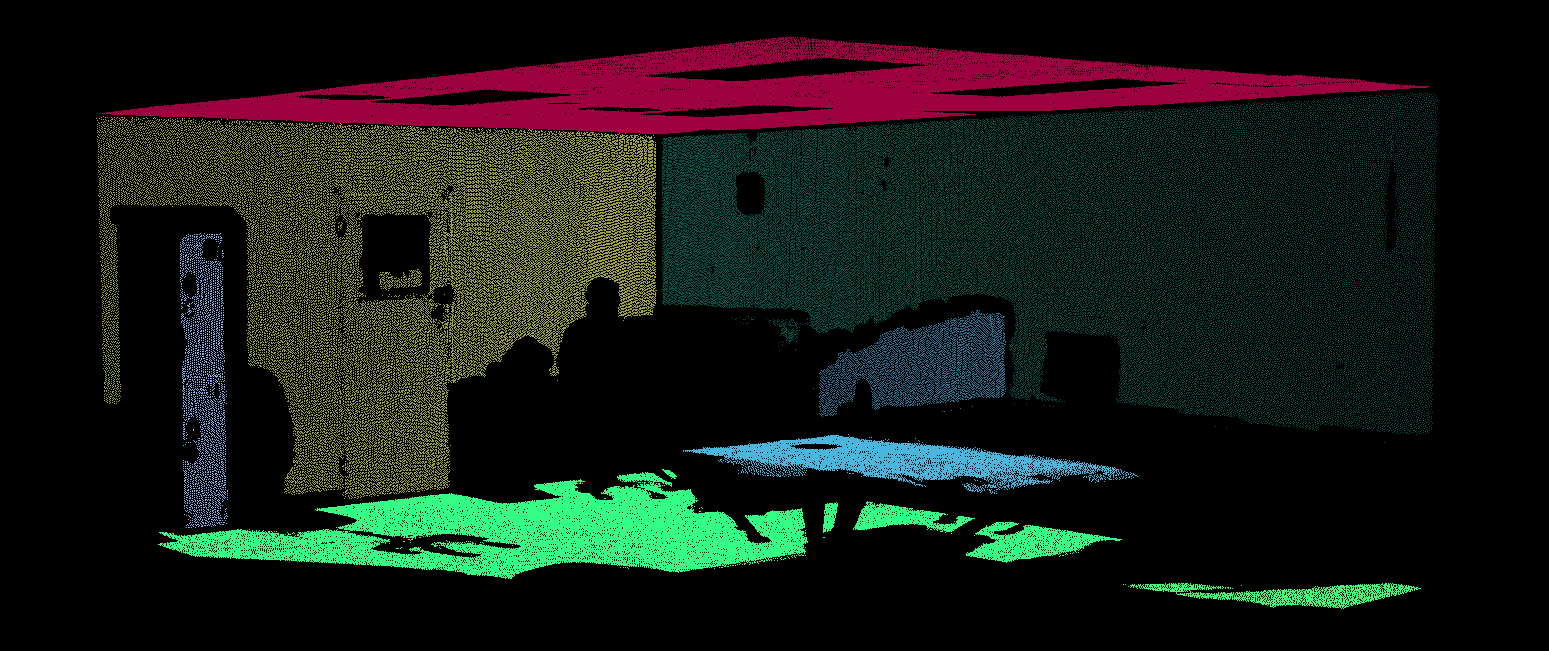
\includegraphics[width=1\linewidth]{Includes/images/RegionGrowing/neighbours-200}
			\caption{Number of Neighbours = 200}
			\label{fig:neighbours-200}
		\end{figure}

		The final parameters, as shown in the constants.h file, are as follows:

		\begin{lstlisting}
int MinClusterSize = 5000;
int NumberOfNeighbours = 40;
float SmoothnessThreshold = (1.0 * M_PI / 180);
float CurvatureThreshold = 1.0;
		\end{lstlisting}
			
			\begin{figure}[H]
				\centering
				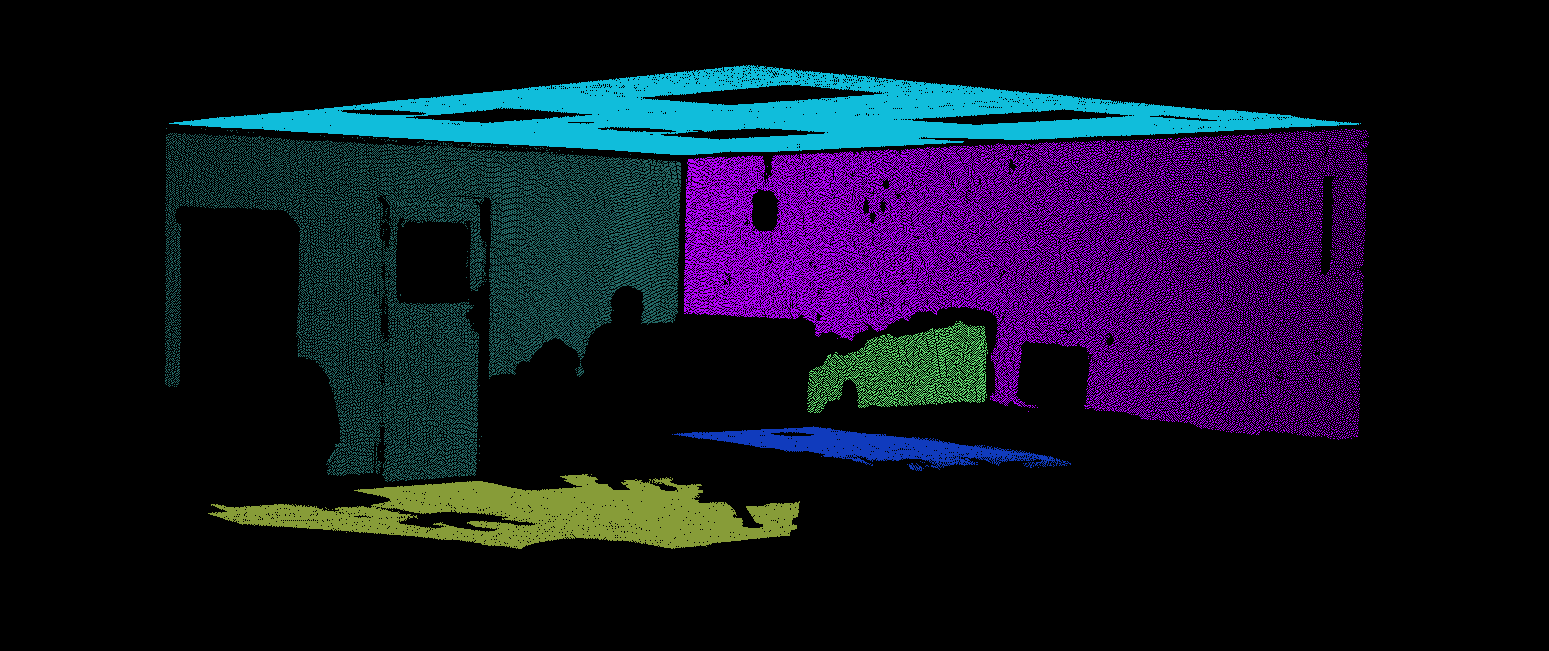
\includegraphics[width=1\linewidth]{Includes/images/RegionGrowing/Final}
				\caption{Final results of region growing}
				\label{fig:Final}
			\end{figure}
 
	
			The segmentation of the point cloud is the most time consuming function in the whole process, taking up on average 80\% of total run-time.
			
			Once again the speed of the process depends greatly on the parameters set
		
		

	\section{Surface Extraction}
	
	It is immediately evident in Figure \ref{fig:min-size=100} that there are too many small segments that are not necessary and irreverent to the final output. So it becomes necessary to filter these segments out. The first obvious step is to up the minimum cluster size like in figure \ref{fig:min-size=5000}. But even with the larger cluster size There are still a number of segments that need to be filtered out.
	
	To begin this, a array of the segments is created after the region growing has taken place.


	\subsection{Segment selection}
		The array of segments created in the segmentation section of the program is not entirely useful due to the fact that it contains segments all the segments.
		
		Most of the segments are small cluttering objects, like sides of desks of tops of tables. In process of trying to extract the boundaries of a room all this clutter is unnecessary, so we need to filter it out somehow.
		\subsubsection{filtering out Horizontal and Vertical surfaces}
		\label{Filtering}
			To start this process, the array of segments is split up into two separate arrays, horizontal segments and vertical segments. This is done by iterating through the segments and deciding which category they fall under.
			
			A plane is fitted to the segment using the RANSAC method outlined in section \ref{RANSAC expl}. Now the orientation of the segment can be determined from the coefficients $a$, $b$, and $c$ of the planes equation.
			
			\begin{equation}
			ax + by + cz = d  \quad\quad
			\vec{n}_{segment} = \begin{bmatrix}a\\b\\c\end{bmatrix}
			\end{equation}
			
			Once the normal to the segment is determined it is compares to a known vertical vector $\vec{v}$. 
			
			\begin{equation}
			\vec{v} = \begin{bmatrix}0\\0\\1\end{bmatrix}
			\end{equation}
			
			The angle between the two vectors is then the deviation the normal has from vertical and can be thought of as the angle the segment has from vertical. The angle is found using the dot product:
			\label{DotProdSec}
			\begin{equation}
			\vec{n}_{segment}\cdot \vec{v} = \norm{\vec{n}_{segment}} \norm{\vec{v}} cos \theta
			\end{equation}
			\begin{figure}[H]
				\centering
				\includegraphics[width=0.4\linewidth]{"Includes/images/normal to plane"}
				\caption{The deflection of the plane normal from vertical}
				\label{fig:normaltoplane}
			\end{figure}

			
			Solving for $\theta$ gives us the angle between the segment and vertical. From here it is easy to decide if a segment is horizontal or vertical, by seeing if $\theta$ is closer to 0\textdegree/180\textdegree or 90\textdegree.
			
			\begin{figure}[H]
				\centering
				\includegraphics[width=1\linewidth]{"Includes/images/SEG Select/CutDown-Vert"}
				\caption{Vertical Segments Before Filtering}
				\label{fig:CutDown-Vert}
			\end{figure}
			
			\begin{figure}[H]
				\centering
				\includegraphics[width=1\linewidth]{"Includes/images/SEG Select/CutDown-HOR"}
				\caption{Horizontal Segments Before Filtering}
				\label{fig:CutDown-HOR}
			\end{figure}
			
		\subsubsection{Filtering of Vertical Segments}
		
			Vertical segments are filtered through two tests:
			\begin{enumerate}
				\item The vertical Extent of the Segment.
				
				\item Another angle check.
			\end{enumerate}
			 
			The vertical extent of the segment is determined by finding the highest, $max = (x_{max},y_{max},z_{max})$, and lowest, $min = (x_{min},y_{minx},z_{min})$ , points and getting the distance between them:
			
			\begin{equation}
			Vertical \: Extent = \sqrt{(x_{max} - x_{min})^2+(y_{max} - y_{min})^2+(z_{max} - z_{min})^2}
			\end{equation}
			
			If the vertical extent of a segment is less that 1m the segment is removed on the basis that it is to small. And does not represent a wall.
			
			The selection based on Angle is simply an extension of the previous method for splitting the the segments based on orientation, but with a much more strict angle defining vertical, $\theta$ must fall within $\pm$10\textdegree of 90\textdegree, i.e. the segment must be within a 10\textdegree of perfectly vertical:
			
			\begin{equation}
			80\textdegree < \theta < 100\textdegree
			\end{equation}
			


			
			\subsubsection{Filtering of the Horizontal Segments}
			
			When deciding what is the roof and what is the floor in the whole point cloud a reasonable assumption to make is that the highest and lowest segments are the roof and floor respectively.
			
			To find the highest and lowest segments is fairly simple. While looping through all the horizontal segments determine which segment has the highest average $z$ value and the lowest average $z$ value. These two segments are added to the filtered vertical segments in an array called Extent\_Clusters.
			
			The Extent\_Clusters array contains only the outer most segments, essentially the roof, floor and walls.
			
			

			
	\section{Model Generation}
		The model generation section of this project is where the planar segments are turned into vertices's and faces so that they can be written to an obj file.
		
		\subsection{Boundaries of Segments}
		\label{boundaries}
			Step 1 in this process is to get the Oriented Bounding boxes of each of the segments. because the segments are planar the bounding boxes are also planar. This means that when a 3D cube is fitted to the segment there are only 4 unique points representing the cube as opposed to 8.
			
			The 4 duplicate points are therefore removed leaving 4 points that are coplanar to the segment to represent the boundary of the segment as shown in Figure \ref{fig:BOundingBox}.
		
			\begin{figure}[H]
				\centering
				\includegraphics[width=1\linewidth]{"Includes/images/Bounding Box/BOunding Box"}
				\caption{The 4 Boundary points of the segment indicated by the red circles}
				\label{fig:BOundingBox}
			\end{figure}
			It is these coplanar boundary points that are adjusted to the corners of the room.
			
		\subsection{Plane with Plane intersection}
		\label{planeInterResults}
			As we have planes fitted to each segment from earlier in section \ref{Filtering} time can be saved by not fitting them again.
			
			For this section two loops are run inside each other, iterating over the array Extent\_Clusters. This makes it possible to intersect all the segments with each other, but also introduces the issue of the program attempting to intersect the same plane with itself of parallel planes with themselves, resulting in lines of intersection way off towards infinity of just errors.\\
			\\
			To solve this the same function that checks the angle between the plane normal and vertical (section \ref{DotProdSec}) is used to check the angle between the two planes. If this angle is less than 15\textdegree\: then that pair of segments is skipped.
			
			If the two segments pass this test, then they are intersected using the method in section \ref{plane-planeInter} and a line of intersection is returned.
			
		\subsection{Adjusting the boundary points through\\ Extrusion}
		\label{Extrusion}
			There are 4 points essentially defining each segment, it is these 4 points that are extruded so that the segment representing a wall of floor actually represents the full extent of that wall or floor. To do this a series of adjustments are applied to the boundary points so that they work their way outward towards the corners of the room. This is done using the Projection function.
			
			Only one of the segments boundary points are projected because all segments will meet twice, due to the two nested loops running through all segments each. This means that the first loops segment boundaries are adjusted with reference to the second loop, and the second loops segment boundaries are never adjusted.\\
			\\
			The Projection function is provided with only 2 objects, the line of intersection that was created earlier, and the boundaries points that were created in \ref{boundaries}. Note that in the line of intersection computation the angle between the two segments is checked as explained in \ref{planeInterResults}.
			
			The Projection function projects the closest two points, determined using the method in Section \ref{DistanceOfPointToLine}, to the line of intersection between the who segments.
			
			This process is graphically shown in Figure \ref{fig:4Adjust},  sub-figure (a) shows the first iteration, (b) shows the second, and so on.
			
			The two red points circled in each of the figures are the closest two points to the line of intersection. These points are projected onto the line of intersection, this projection is shown by the arrows.
			
			\begin{figure}[p] 
				\centering
				\begin{subfigure}[b]{0.49\linewidth}
					\centering
					\includegraphics[width=1\linewidth]{"Includes/images/Project Points/F-1"} 
					\caption{First iteration} 
					\label{fig4Adjust:a} 
					\vspace{4ex}
				\end{subfigure}
				\begin{subfigure}[b]{0.49\linewidth}
					\centering
					\includegraphics[width=1\linewidth]{"Includes/images/Project Points/F-2"} 
					\caption{Second iteration} 
					\label{fig4Adjust:b} 
					\vspace{4ex}
				\end{subfigure} 
				\begin{subfigure}[b]{0.49\linewidth}
					\centering
					\includegraphics[width=1\linewidth]{"Includes/images/Project Points/F-3"} 
					\caption{Third iteration} 
					\label{fig4Adjust:c} 
				\end{subfigure}
				\begin{subfigure}[b]{0.49\linewidth}
					\centering
					\includegraphics[width=1\linewidth]{"Includes/images/Project Points/F-4"} 
					\caption{Fourth iteration} 
					\label{fig4Adjust:d} 
				\end{subfigure} 
				\caption{The iterative extrusion of boundary points to the lines of intersection}
				\label{fig:4Adjust} 
			\end{figure}
			
			Figure \ref{fig:F-5} shows the complete path taken by each boundary point as it is projected onto each line of intersection. The blue points are starting positions of the boundary points as calculated in \ref{boundaries}. These points after projection result in the red points.

			\begin{figure}[H]
				\centering
				\includegraphics[width=0.6\linewidth]{"Includes/images/Project Points/F-5"}
				\caption{The final positions of the boundary points after Extrusion represented by the Red points and original positions represented by the Blue points}
				\label{fig:F-5}
			\end{figure}
			
		\subsection{Dealing with Duplicate Corner Points}
			Due to the fact that the corner of a room is created by the intersection of 3 segment planes, there will be 3 boundary points at each corner, one for each segments plane.
			
			These points do not always have the same value and usually vary by up to 5cm. To solve this issue of multiple points where there should be one point, a simple clustering algorithm is run to group together points close together.
			
			The clustering algorithm simply take points that are within 5cm of each other and places them in an array defining that corner.
			
			The array is then averaged and that average value set as the value of the 3 corner points. Resulting in 1 point representing a corner.
			
			\begin{figure}
				\centering
				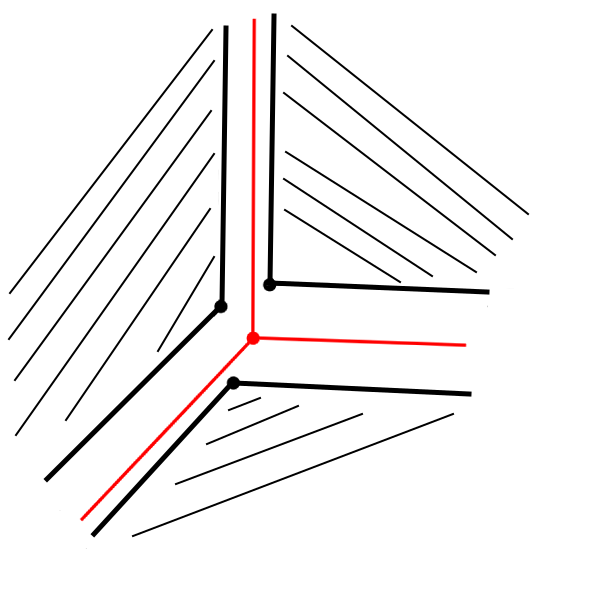
\includegraphics[width=0.7\linewidth]{Includes/images/CornerAveraging}
				\caption{Duplicate Cornet points shown in black, averaged corner shown in red.}
				\label{fig:CornerAveraging}
			\end{figure}
			
			Figure \ref{fig:CornerAveraging} shows in black what the corner of a room without averaged points will look like. The red point and lines shows what the corner will look like after averaging.


		\subsection{Creating the B-rep Model from the Adjusted Boundary Points}
			Creating the boundary representation model from the the averaged, Adjusted boundary points is the last part of this project. The model is created by iterating through each set of boundary points and writing each one of them as a separate object to an OBJ file as outlined in Section \ref{makeOBJfile}. Resulting is a simple boundary representation of the original laser scan.
			
			The output of the B-rep model are lines representing the edges of the room as seen in Figure \ref{fig:full2}, \ref{fig:full3} and \ref{fig:untitled}.
			
			
			The results of different point clouds can be found in Appendix B.
			
			
			
			\begin{figure}[H]
			\centering
			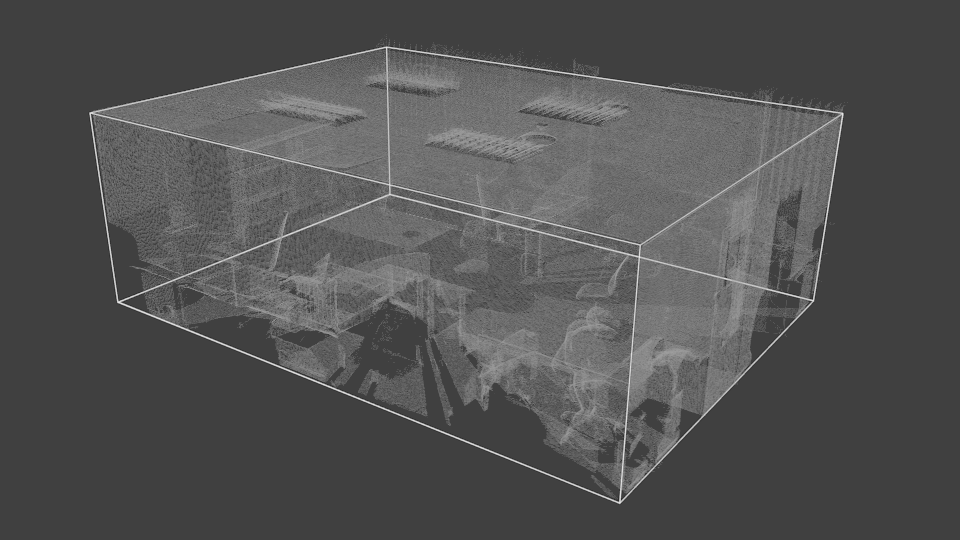
\includegraphics[width=1\linewidth]{Includes/images/f/full4}
			\caption{Final Boundary representation of the room looking from the front right corner of the room}
			\label{fig:full2}
			\end{figure}

			\begin{figure}[H]
			\centering
			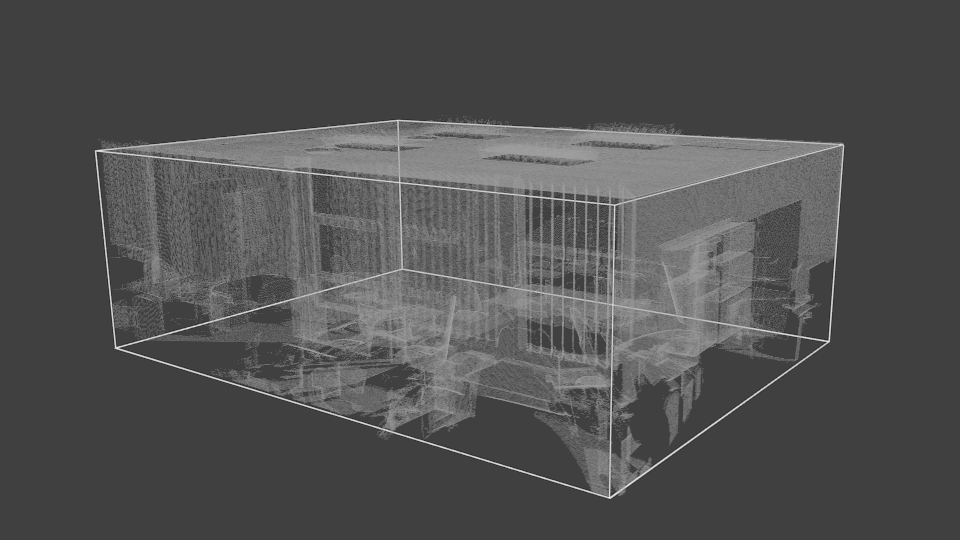
\includegraphics[width=1\linewidth]{Includes/images/f/full2}
			\caption{Final Boundary representation of the room looking from the back left corner of the room}
			\label{fig:full3}
			\end{figure}
			
			
			\begin{figure}[H]
			\centering
			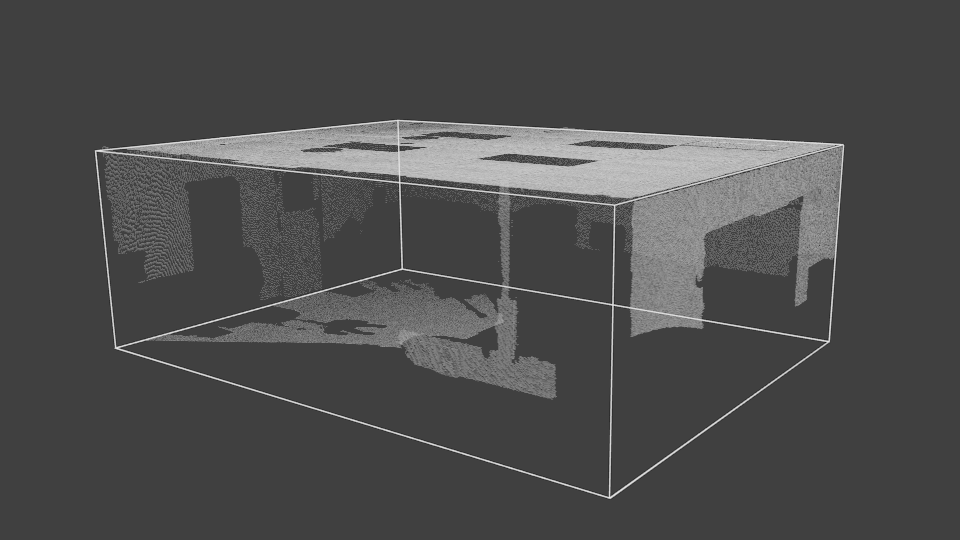
\includegraphics[width=1\linewidth]{Includes/images/f/untitled}
			\caption{Final Boundary representation of the room with segmented cloud}
			\label{fig:untitled}
			\end{figure}
			
			\begin{figure}[H]
			\centering
			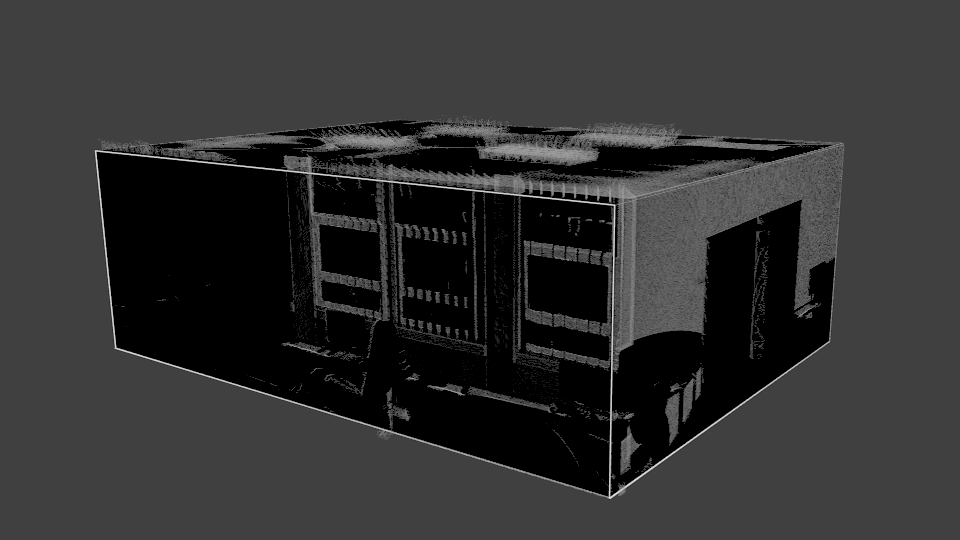
\includegraphics[width=1\linewidth]{Includes/images/f/full5}
			\caption{Full cloud with Boundary Representation looking from the front right corner of the room}
			\label{fig:full5}
			\end{figure}
			
			\begin{figure}[H]
			\centering
			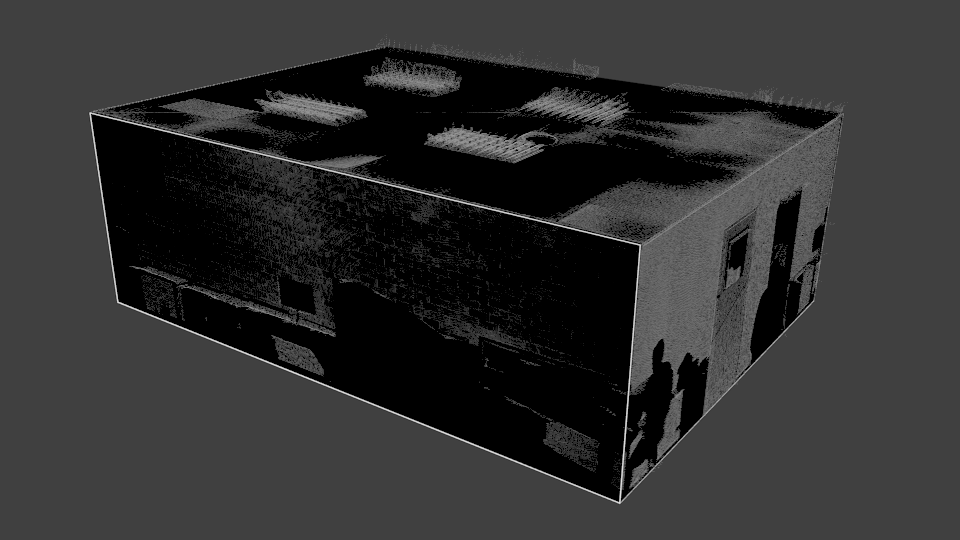
\includegraphics[width=1\linewidth]{Includes/images/f/full6}
			\caption{Full cloud with Boundary Representation looking from the back left corner of the room}
			\label{fig:full6}
			\end{figure}


			

			
			